\documentclass[a4paper,10pt]{article}
 
\usepackage[T1]{fontenc}
\usepackage[utf8]{inputenc}
\usepackage{graphicx}
\usepackage{xcolor, colortbl}
\usepackage{caption}
\usepackage{listings}
\usepackage{wrapfig} 
\usepackage{tabu} % For coloring single row of table
\usepackage{scrextend}

\renewcommand\familydefault{\sfdefault} 
\usepackage{tgheros}
\usepackage[defaultmono]{droidmono}

\usepackage{amsmath,amssymb,amsthm,textcomp}
\usepackage{enumerate}
\usepackage{multicol}
\usepackage{tikz}

\usepackage{geometry}
\usepackage{trace}
\usepackage{tcolorbox}
\usepackage{tabularx}
\usepackage{accsupp}% http://ctan.org/pkg/accsupp


\tcbuselibrary{listings,skins} % For lstlisting

\geometry{total={210mm,297mm},
left=25mm,right=25mm,%
bindingoffset=0mm, top=20mm,bottom=20mm}


% For coloring single row in table
\def\zapcolorreset{\let\reset@color\relax\ignorespaces}
\def\colorrows#1{\noalign{\aftergroup\zapcolorreset#1}\ignorespaces}

\newcommand{\linia}{\rule{\linewidth}{0.5pt}}
\newcommand{\ano}{\text{1}}

% custom theorems if needed
\newtheoremstyle{mytheor}
    {1ex}{1ex}{\normalfont}{0pt}{\scshape}{.}{1ex}
    {{\thmname{#1 }}{\thmnumber{#2}}{\thmnote{ (#3)}}}

\theoremstyle{mytheor}
\newtheorem{defi}{Definition}

% my own titles
\makeatletter
\renewcommand{\maketitle}{
\begin{center}
\vspace{2ex}
{\huge \textsc{\@title}}
\vspace{1ex}
\\
Department of Electronics and Communication Engineering \\
Indian Institute of Technology, Roorkee
\linia\\
ECN 104 \hfill Digital Logic Design
\vspace{4ex}
\end{center}
}
\makeatother
%%%

% custom footers and headers
\usepackage{fancyhdr}
\pagestyle{fancy}
\lhead{}
\chead{}
\rhead{}
\lfoot{Assignment \ano - Introduction to Verilog}
\cfoot{}
\rfoot{Page \thepage}
\renewcommand{\headrulewidth}{0pt}
\renewcommand{\footrulewidth}{0pt}
%

\definecolor{vgreen}{RGB}{104,180,104}
\definecolor{vblue}{RGB}{49,49,255}
\definecolor{vorange}{RGB}{255,143,102}

\makeatletter
\newcommand*\@lbracket{[}
\newcommand*\@rbracket{]}
\newcommand*\@colon{:}
\newcommand*\colorIndex{%
    \edef\@temp{\the\lst@token}%
    \ifx\@temp\@lbracket \color{black}%
    \else\ifx\@temp\@rbracket \color{black}%
    \else\ifx\@temp\@colon \color{black}%
    \else \color{vorange}%
    \fi\fi\fi
}
\makeatother

\definecolor{codebg}{RGB}{250,250,240} 
\definecolor{greatblue}{RGB}{91,155,215} 

% Set up caption and labels for lstlistings
\DeclareCaptionFont{white}{\color{white}}
\DeclareCaptionFormat{listing}{\colorbox{greatblue}{\parbox{\textwidth}{\hspace{1cm}#1#2#3}}}
\captionsetup[lstlisting]{format=listing,labelfont=white,textfont=white}

\renewcommand{\thelstnumber}{% Line number printing mechanism
  \protect\BeginAccSupp{ActualText={}}\arabic{lstnumber}\protect\EndAccSupp{}%
}

\def\backtick{\char18} 
\lstdefinestyle{verilog-style}
{
    %columns=fullflexible, 
    language=Verilog,
    basicstyle=\small\ttfamily,
    keywordstyle=\color{vblue},
    identifierstyle=\color{black},
    commentstyle=\color{vgreen},
    numbers=left, 
    numberstyle=\color{gray},  
    numbersep=10pt,
    moredelim=*[s][\colorIndex]{[}{]},
    literate=*{:}{:}1, 
    backgroundcolor=\color{codebg},
    framexrightmargin=0.09cm, 
    framexleftmargin=-0.09cm,
    frame=trbl,
    upquote=true, 
    framerule=0pt,
    keepspaces=true
}

\newcommand{
  \insertverilog}[3]{
  \lstinputlisting[label=#2, caption=#3, style={verilog-style}]{#1}
}

% Command for problem
\newcounter{problemNumber}
\setcounter{problemNumber}{1}
\newcommand {
  \insertProblem}[1]{
  \vspace{0.5cm}
  \hrule
  \vspace{0.3cm}

  {\color{greatblue}\textbf{\large{Problem \theproblemNumber}}}
  \vspace{2pt}\\#1

  \addtocounter{problemNumber}{1}
  \vspace{0.2cm}
  \hrule  
  \vspace{0.5cm}
}


%%%----------%%%----------%%%----------%%%----------%%%
% Command for creating a resource box
\newcommand{\resourcebox}[2]{
  \fbox{%
    \parbox{0.5\textwidth}{%
      \text{#1}
    }%
  } 
}


%%%----------%%%----------%%%----------%%%----------%%%

\makeatletter
\def\lst@outputspace{{\ifx\lst@bkgcolor\empty\color{white}\else\lst@bkgcolor\fi\lst@visiblespace}}
\makeatother


%%%----------%%%----------%%%----------%%%----------%%%
\begin{document}

\title{Assignment \ano \\ Introduction to Verilog}

\maketitle

\section*{Hardware Description Languages}
A hardware description language (HDL) is a convenient, device and technology independent way of representing digital logic. HDLs are helpful describing, simulating and verifying digital circuits.

\subsection*{Why not use C/C++, Java...?} 
C/C++, Java etc. are programming languages which are very good at what they were designed for, that is programming. However, describing digital circuits in a programming language is difficult and often confusing as it needs more specifications on 'How To' alongside 'What To'.

For example, let's say you want to add 4 1-bit numbers. Now, if you were programming in C/C++, you would have simply written RESULT=a+b+c+d and left the rest to your compiler. But when implementing this logic on hardware, there are more than one ways to do it. You can either cascade three adders or make an adder-tree using three adders. Now both of these implementations have different delays and thus you must have the freedom to decide which one to use. No doubt you could achieve whichever implementation you want by writing some extra lines of C++ to specify exactly what you want, but, as the problem complexity grows, this extra effort to exactly specify what we want grows drastically. This led to development of HDLs where WYWIWYG(What You Write Is What You Get). NOTE: Although this may not be the case if you are lazy and leave ambiguity in your HDL code leaving it to the synthesizing software to decide upon. 

\subsection*{Which HDL to use?}
Many hardware description languages are available today. Each of them is different from the other in terms of functionality, semantics and grammar. In this course however, we will stick to Verilog  2001.

\section*{Using Verilog 2001}
As a beginner, we are going to describe and simulate simple combinational circuits with Verilog.

\section*{Design Flow}  

\begin{figure}[h] \centering 
  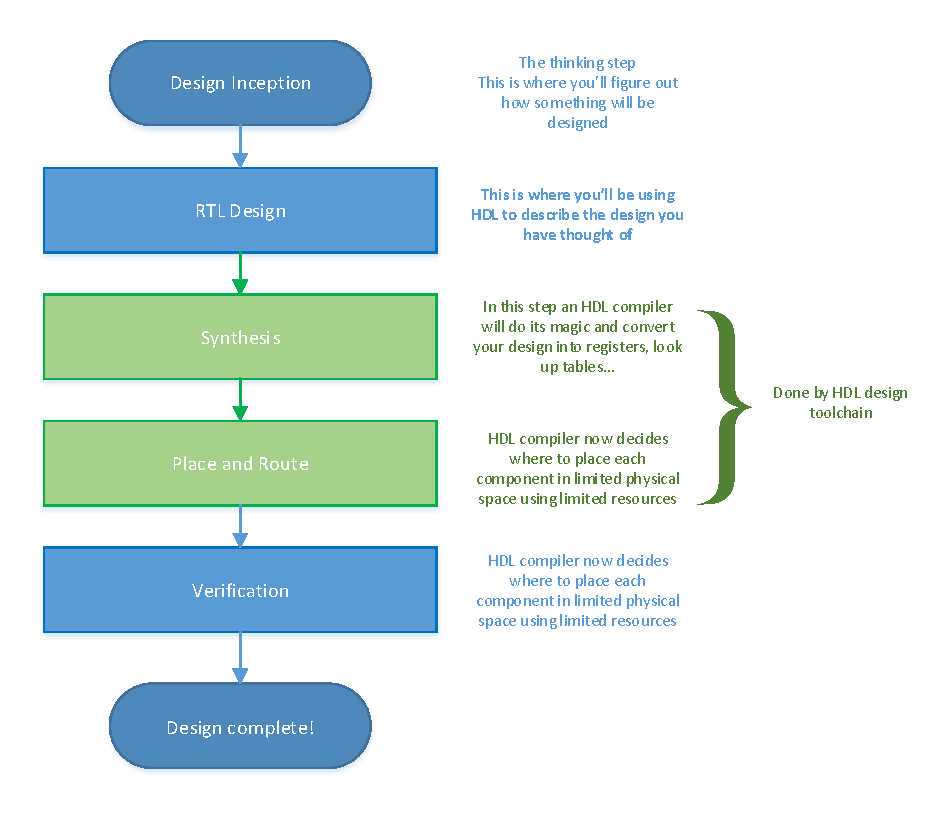
\includegraphics[width=\linewidth]{./resources/hdl_design_flow.pdf}
  \caption{Basic design flow of a design from its inception to implementation.}
  \label{Fig:bst_sample_names}
\end{figure} 

\section*{Verilog Syntax}
\subsection*{Modules}
Module, the basic building block in Verilog, helps in organizing and structuring designs in logical and human readable form. A module can be considered as analogous to functions in programming languages(NOT EXACTLY though. Functions, by definition, act in BATCH MODE i.e, you give them inputs and get output after sometime. Batch mode here means before getting the output once, you can't send in new inputs. But in HDL, you may write PIPELINED modules. Pipelining can be understood by the working of a car assembly line. The job is divided into smaller sections. Now while a car is being painted, some other cars may be in the welding and testing sections. This naturally leads to faster production of cars if the company has a large order.) Basic structure of a Verilog module is given in Listing \ref{sample-module-bare} 

\insertverilog{./verilog_files/module.v}{sample-module-bare}{\text{Sample module indicating its structure}}

An example of AND gate is given in Listing \ref{and-gate-module-sample}
\insertverilog{./verilog_files/andGate.v}{and-gate-module-sample}{\text{Illustrative AND gate module}}

\subsection*{Instantiating modules}
The process of creating objects of modules is called instantiation in Verilog. Modules are like blueprints and instantiating them means constructing hardware using the blueprints.
  
\insertverilog{./verilog_files/AndGate3.v}{sample-module}{\text{Illustrative AND gate module}} 
\subsection*{Comments}
Comments in Verilog are of two kinds:
\subsubsection*{Single Line Comment}
Two forward slashes represents begining of a single line comment in Verilog, anything in a line after those two characters will ignored by the compiler
\insertverilog{./verilog_files/singleLineComment.v}{single-line-comment}{\text{Single line comment}} 

\subsubsection*{Block Comment}
Block comments in verilog are used to comment a block of code, they start with `/*' and ends with `*/'. Anything between these two character sequences will be ignored by the compiler.
\insertverilog{./verilog_files/blockComment.v}{block-comment}{\text{Block
    comment}}

\subsection*{Numerical Literals}
\subsubsection*{Sized Numbers}
To represent digital circuits accurately Verilog allows defining
numbers of fixed size. These numbers have the following format:
\begin{center}
  <size>'<character for base><number>
\end{center}

For example:
\insertverilog{./verilog_files/sizedNumbers.v}{sized-numbers}{\text{Example of sized numbers}}
 
\subsubsection*{Unisized Numbers}
Verilog also includes support for unsized numbers. These numbers are
assumed to be of a particular size depending on the
compiler/machine.

\subsection*{Constants}
Global constants can be declared in Verilog. When Verilog code is processed all these constants will be replaced by their respective values. NOTE: Verilog constants always starts with backtick ` ${}^{\backprime}$ '. 
\insertverilog{./verilog_files/constants.v}{constants}{\text{Declaration and use of constants}}

\subsection*{Wires}

\begin{figure}[!h] \centering  
  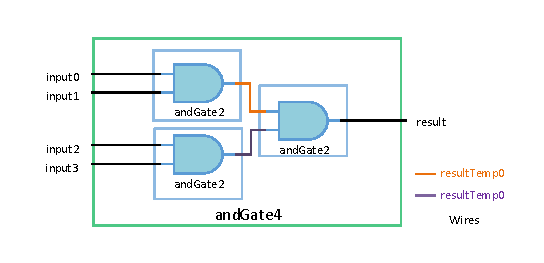
\includegraphics[width=\linewidth]{./resources/andGate4_representation.pdf}
  \caption{Gate level representation of code in Listing \ref{andGate4-wire}.} 
  \label{Fig:andGate4-representation}
\end{figure}

Wires are something very important in verilog. Use of wires in Verilog is for what wires are used in real life ... to connect two things electrically! Wires will be used extensively in future assignments to connect two modules, registers and even wires together. This concept is explained using Listing \ref{constants} where wires are used to connect the output of two 2-input AND gates to inputs of single 2-input AND gates. Gate level diagram of which is shown in Fig. \ref{Fig:andGate4-representation}.

\insertverilog{./verilog_files/andGate4.v}{andGate4-wire}{\text{Use of wires to connect output of one module to input of another}}

\subsubsection*{Vectors}
Verilog supports declaration of vectors to represent a group of wires (or registers which will be explained later). Vectors are declared by specifying their type, range and then their name:
\begin{center}
  <type> <range> <name>;
\end{center}

Example declaration of 6 bit wide vector of type wire:
\begin{center}
  {\color{blue} wire} [{\color{orange}5}:{\color{orange}0}] new\_wire; {\color{vgreen}// Both the range specifier digits are inclusive}
\end{center}

Here new\_wire[{\color{orange}5}] is MSB while new\_wire[{\color{orange}0}] is LSB.

\subsubsection*{Part Select}
What if you wanted to access $2^{nd}$, $3^{rd}$ and $4^{th}$ elements of a vector? This is when part select of verilog will help. Part select in Verilog allows extraction of a smaller vector from an existing vector.\\ 
\vspace{0.2cm}\\
Example:
\insertverilog{./verilog_files/bitExtract.v}{bit-extract}{\text{Using bit extract to extract lower, higher and middle 16 bits from a 32 bit input}}

\begin{figure}[!h] \centering  
  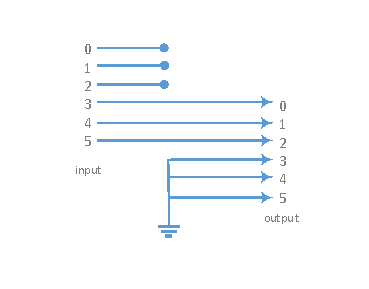
\includegraphics[width=0.45\linewidth]{./resources/shiftUsingWires_representation.pdf}
  \caption{A shift right by 3 element design for bus width of 6.} 
  \label{Fig:shiftUsingWires-representation}
\end{figure}
\insertProblem{ Shift operation is one of the important operation in a digital system. Various different designs exist for performing shifts of arbitrary amount within a range(Search the internet for Barrel Shifters for one implementation). But, a fixed amount shifter (e.g. a shift by 5 element) is extremely easy to implement. This is done by moving connections from input to output along the desired direction by the desired amount. An example of which is given in Fig. \ref{Fig:shiftUsingWires-representation} 

  Write a Verilog module which uses part select, takes a 32bit vector as input named \textsc{inputSignal} and outputs a 32bit vector \textsc{result} which is simply inputSignal shifted by 5 towards left. Use \textsc{testbench{\ano}.{\theproblemNumber}.v} to verify the output. (\textit{Hint: Similar to part select, Verilog supports part assign which allows assigning values to a part of a vector})}
%

\subsection*{Operators}
Verilog supports a wide range of operators to represent mathematical operations. These are high level representation of what later would be converted to a gate level implementation by your HDL compiler.

\begin{table}[h]
  \begin{center}
    \label{Table:operators-table}
    \caption{List of common operators used in Verilog}
    \renewcommand{\arraystretch}{1.1}
    \begin{tabularx}{.8\textwidth}{|X|X|X|} 
      \hline
      \rowcolor{greatblue}
      \color{white}  Operator & \color{white}Description & \color{white}Functional Group \\
      %  \colorrows{\color{black}} 
      \hline
      \text{[]} & bit select or part select &  \\
      
      \hline
      \text{()} & parenthesis &  \\
      
      \hline
      \text{!} & negation &  logical\\
      \text{\textasciitilde} & negation &  bit\-wise\\
      \text{\&} & reduction AND & reduction \\
      \text{\textbar} & reduction OR & reduction \\
      \text{\textasciitilde\&} & reduction NAND & reduction \\
      \text{\textasciitilde\textbar} & reduction NOR & reduction \\
      $^\wedge$ & reduction XOR & reduction \\
      \textasciitilde$^\wedge$ or $^\wedge$\textasciitilde & reduction XNOR & reduction \\
      \hline
      $+$ & Unary Plus (plus sign) & airthmetic \\
      $-$ & Unary minus (minus sign) & \\
      \hline
      $*$ & multiply & airthmetic \\
      $/$ & divide &  \\
      \% & modulus &  \\
      \hline
      $+$ & Binary Plus & airthmetic \\
      $-$ & Binary minus &  \\
      \hline
      $<<$ & shift left & shift \\
      $>>$ & shift right &  \\
      \hline
      $>$ & greater than & relational \\
      $>=$  & greater than or equal to & \\
      $<$ & less than  & \\
      $<=$ & less than or equal to & \\
      \hline  
      $==$ & case equality & equality \\
      $!=$  & case inequality & \\
      \hline
      \text{\&} & bitwise AND & bitwise \\
      \text{\textbar} & bitwise OR & \\
      \text{\textasciitilde} & bitwise XOR & \\
      \hline
    \end{tabularx}
  \end{center}
\end{table}

\subsubsection*{Airthmetic Operators}
Veriog allows use of various airthmetic operators to perform
calculations on vectors (wires \& reg). Following example shows its
usage:
\insertverilog{./verilog_files/airthmeticOperators.v}{airthmetic-operators}{\text{Functioning of airthmetic operator}}

\insertProblem{Hirerarichal design is often helpful in verifying large project easily by verifying each individual module seperately. Make a module for 2 input NAND gate. Now, make a 2 input And gate by connecting both the input of NAND gate to another NAND gate. Use \textsc{testbench{\ano}.{\theproblemNumber}.v} to verify the output.}


\subsubsection*{Reduction Operators}
Reduction operators in Verilog reduces a vector into a single
bit by repeatedly performing a specified operation. Following example 
explains its usage: 
\insertverilog{./verilog_files/reductionOperators.v}{reduction-operators}{\text{Functioning of reduction operator}}

\insertProblem {
  Reduction operators are often used when some computation has to be performed on complete signal, particular example of which is calculating XOR of a signal to get its parity bit. Even parity bit of a signal is 1 if signal has odd number of 1 and 0 if number of 1s is even, similarily odd parity bit of number is 1 if signal has even number of 1 and 0 if number of 1s is odd.

  Write a Verilog module which uses reduction operator, takes a 32bit vector as input named \textsc{signal}, two single bit output named \textsc{parityEven} and \textsc{parityOdd}. Use \textsc{testbench{\ano}.{\theproblemNumber}.v} to verify output. (\textit{Hint: Calculating XOR of all bits of a signal gives even parity of the signal.})
}

\subsubsection*{Relational Operators}
Relational operators in verilog are used to compare two values, usage
of all four type of relational operators supported by Verilog are
given in Listing \ref{relational-operators}.
\insertverilog{./verilog_files/relationalOperators.v}{relational-operators}{\text{Functioning of relational operator}}
  
\subsubsection*{Logical Operators}
Logical operators are used in conjuction with relational and equality
to perform multiple comparisions within a single expression.
Example usage of logical operators are provided in \ref{logical-operators}.
\insertverilog{./verilog_files/logicalOperators.v}{logical-operators}{\text{Functioning of logical operator}}

\subsubsection*{Bitwise and Shift Operators}
Verilog Bitwise and Shift operators works in the same way as they work
in Java, except that in Verilog only left shift (\textbf{$<<$}) and right shift
(\textbf{$>>$}) are supported.(There is an arithmetic right shift operator too which can be searched on the internet for details!)

\begin{figure}[!h] \centering  
  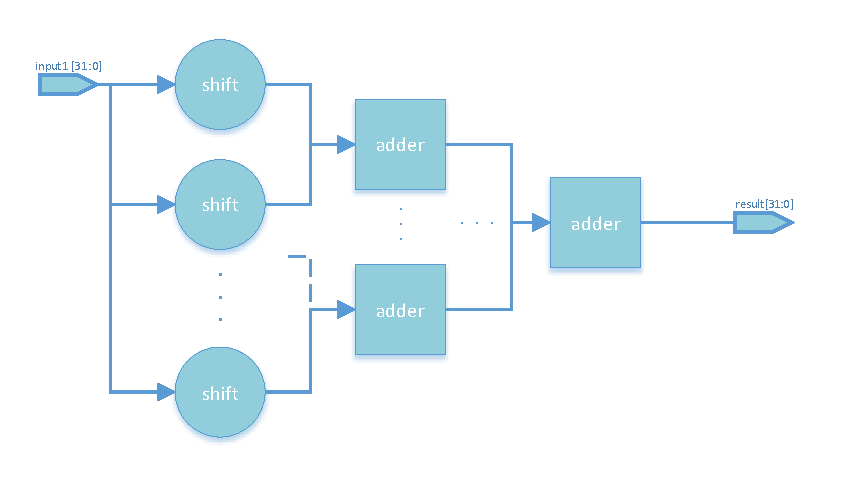
\includegraphics[width=0.9\linewidth]{./resources/shift_and_add_representation.pdf}
  \caption{RTL schematic for Problem 4. \textbf{Note:} This is representative RTL schematic, solution to the problem will have fixed number of shift and add blocks.} 
  \label{Fig:problem-4-RTL} 
\end{figure}    

\insertProblem {
  Multiplying using digital logic is a challenging task, one very intuitive approach is to use `shift-and-add approach'; in this method, two binary numbers are multiplied by shifting one and adding to other. This is repeated till the desired multiplication is obtained. This approach is described here: \begin{center}https://en.wikipedia.org/wiki/Binary\_multiplier\#Multiplication\_basics\end{center} 
  
    Write a module for multiplying a 32-bit binary number by 10(4'b1010 in binary) without using the multiply operator. Assume the input is such that output doesn't overflow. Use \textsc{testbench{\ano}.{\theproblemNumber}.v} to verify output. RTL schematic of your module should resemble Fig. \ref{Fig:problem-4-RTL}.
}

\section*{References}
\begin{itemize}
  \small 
  \item http://cva.stanford.edu/people/davidbbs/classes/ee108a/winter0607\%20labs/ee108a\_nham\_intro\_to\_verilog.pdf
  \item Verilog HDL: A Guide to Digital Design and Synthesis, Second Edition. By Samir Palnitkar. Publisher: Prentice Hall PTR. Pub Date: February 21, 2003. ISBN: 0-13-044911-3
  \item https://www.utdallas.edu/{\textasciitilde}akshay.sridharan/index\_files/Page5212.htm
\end{itemize}
\end{document}

